%%%%%%%%%%%%%%%%%%%%%%%%%%%%%%%%%%%%%%%%%%%%%%%%%%%%%%%%%%%%%%%%%%%%%%%%%%%%%%%
% Advanced Networking Assignment 4: Queuing Theory
% Università della Svizzera italiana
% Date: April 7, 2025
%
% This report draws on materials from the textbook:
%   A. Carzaniga, Elements of Queuing Theory, March 5, 2025.
%
% The assignment consists of:
%   1. Determining the maximum external arrival rate r₁ in a network of queues.
%   2. Applying Little's Theorem to an Emergency Room (ER) scenario and discussing waiting room capacity.
%   3. Proving the formula for the average number of customers waiting in an M/M/1 queue.
%   4. Analyzing an M/M/1 queue for a packet transmission link.
%%%%%%%%%%%%%%%%%%%%%%%%%%%%%%%%%%%%%%%%%%%%%%%%%%%%%%%%%%%%%%%%%%%%%%%%%%%%%%%

\documentclass[12pt]{article}
\usepackage{amsmath, amssymb}
\usepackage{geometry}
\usepackage{graphicx}
\usepackage{hyperref}
\usepackage{cleveref}
\geometry{a4paper, margin=1in}
\hypersetup{
    colorlinks=true,
    linkcolor=blue,
    urlcolor=blue,
}

\title{Advanced Networking Assignment 4: Queuing Theory}
\author{Zitian Wang \\ Università della Svizzera italiana}
\date{April 7, 2025}

\begin{document}
\maketitle

%%%%%%%%%%%%%%%%%%%%%%%%%%%%%%%%%%%%%%%%%%%%%%%%%%%%%%%%%%%%%%%%%%%%%%%%%%%%%%%
\section{Maximum Rate Possible in a Network of Queues}

Consider the network of queues shown in figure1
\begin{figure}[htbp]
    \centering
    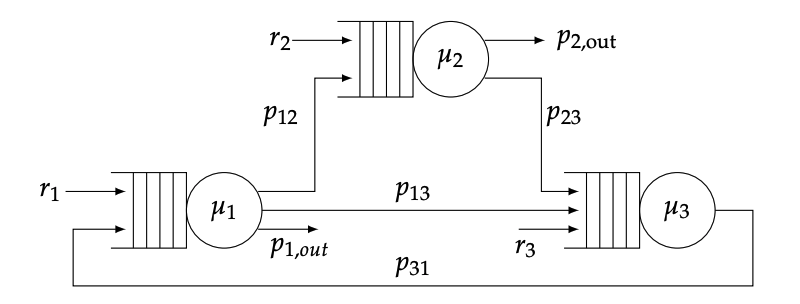
\includegraphics[width=0.8\textwidth]{fig1.png}
    \caption{A network of queues with probabilistic routing.}
\end{figure}
. There are three nodes with the following characteristics:
\begin{itemize}
    \item Each server has a mean service rate of \(\mu = 10\) jobs/sec.
    \item External arrival rates: \(r_2 = 1\) job/sec, \(r_3 = 1\) job/sec, and \(r_1\) is the unknown arrival rate to be determined.
    \item Routing probabilities:
          \begin{itemize}
              \item From node 1: \(p_{12} = 0.8\) (to node 2), \(p_{13} = 0.2\) (to node 3), and \(p_{1,\mathrm{out}}=0\).
              \item From node 2: \(p_{23} = 0.2\) (to node 3) and \(p_{2,\mathrm{out}} = 0.8\).
              \item From node 3: \(p_{31} = 1\) (all jobs are routed back to node 1).
          \end{itemize}
\end{itemize}

Let \(\lambda_1\), \(\lambda_2\), and \(\lambda_3\) denote the total arrival rates at nodes 1, 2, and 3, respectively. Based on the routing and external arrivals, we can establish the following balance equations:
\begin{align}
    \lambda_1 &= r_1 + p_{31}\lambda_3 = r_1 + \lambda_3, \label{eq:node1}\\[1mm]
    \lambda_2 &= r_2 + p_{12}\lambda_1 = 1 + 0.8\,\lambda_1, \label{eq:node2}\\[1mm]
    \lambda_3 &= r_3 + p_{23}\lambda_2 + p_{13}\lambda_1 
               = 1 + 0.2\,\lambda_2 + 0.2\,\lambda_1. \label{eq:node3}
\end{align}

Substituting equation~\eqref{eq:node2} into \eqref{eq:node3} gives:
\[
\lambda_3 = 1 + 0.2\,(1+0.8\,\lambda_1) + 0.2\,\lambda_1 = 1.2 + 0.36\,\lambda_1.
\]
Now substitute this expression into \eqref{eq:node1}:
\[
\lambda_1 = r_1 + (1.2 + 0.36\,\lambda_1).
\]
Solving for \(\lambda_1\):
\begin{align*}
    \lambda_1 - 0.36\,\lambda_1 &= r_1 + 1.2,\\[1mm]
    0.64\,\lambda_1 &= r_1 + 1.2,\\[1mm]
    \lambda_1 &= \frac{r_1 + 1.2}{0.64}.
\end{align*}

Stability of the system requires that for each node the arrival rate must be less than the service rate (\(\lambda_i < 10\) jobs/sec). The most restrictive condition is at node 1:
\[
\frac{r_1 + 1.2}{0.64} < 10 \quad \Rightarrow \quad r_1 + 1.2 < 6.4 \quad \Rightarrow \quad r_1 < 5.2.
\]

\textbf{Conclusion:} To ensure system stability, the external arrival rate \(r_1\) must satisfy
\[
r_1 < 5.2 \quad \text{(jobs/sec)}.
\]

%%%%%%%%%%%%%%%%%%%%%%%%%%%%%%%%%%%%%%%%%%%%%%%%%%%%%%%%%%%%%%%%%%%%%%%%%%%%%%%
\section{Little's Theorem and its Application to the Emergency Room}

In this problem, the following are given:
\begin{itemize}
    \item The mean waiting time in the Emergency Room (ER) is \(W = 3\) hours.
    \item Patients arrive on average every 5 minutes, which implies an arrival rate of:
          \[
          \lambda = \frac{60 \, \text{min/hour}}{5 \, \text{min/patient}} = 12 \, \text{patients/hour}.
          \]
\end{itemize}

Little’s Theorem states that:
\[
L = \lambda\,W,
\]
where \(L\) is the average number of customers (or patients) in the system.

Thus, the average number of patients waiting (or being treated) in the ER is:
\[
L = 12\,\text{patients/hour} \times 3\,\text{hours} = 36\,\text{patients}.
\]

\textbf{Discussion on Waiting Room Capacity:}  
The computed \(L = 36\) represents an \emph{average} value. Due to random fluctuations inherent in queuing systems, there is a nonzero probability of having more than 36 patients at any given time. Therefore, if one requires the waiting room to always accommodate arriving patients (i.e., ensuring zero loss), the capacity would need to be infinite. In practical designs, however, the waiting room is sized to limit the probability of overflow to an acceptably small level.

%%%%%%%%%%%%%%%%%%%%%%%%%%%%%%%%%%%%%%%%%%%%%%%%%%%%%%%%%%%%%%%%%%%%%%%%%%%%%%%
\section{Proof of the M/M/1 Queue Length Formula}

For a standard M/M/1 queue, the stationary distribution (including the customer in service) is given by:
\[
P(N = n) = (1-\rho)\,\rho^n, \quad n \ge 0,
\]
with the utilization \(\rho = \lambda/\mu\). The expected number of customers in the system is:
\[
E[N] = \frac{\rho}{1-\rho}.
\]

Since the server can serve at most one customer at a time, the mean number of customers in service is \(\rho\). Thus, the average number of customers waiting in the queue (excluding the one in service) is:
\[
E[N_Q] = E[N] - \rho = \frac{\rho}{1-\rho} - \rho.
\]

Simplify the expression:
\begin{align*}
E[N_Q] &= \frac{\rho - \rho(1-\rho)}{1-\rho} \\
       &= \frac{\rho - \rho + \rho^2}{1-\rho} \\
       &= \frac{\rho^2}{1-\rho}.
\end{align*}

This completes the proof that:
\[
E[N_Q] = \frac{\rho^2}{1-\rho}.
\]

%%%%%%%%%%%%%%%%%%%%%%%%%%%%%%%%%%%%%%%%%%%%%%%%%%%%%%%%%%%%%%%%%%%%%%%%%%%%%%%
\section{M/M/1 Queue Analysis for a Packet Transmission Link}

Consider a transmission link with the following parameters:
\begin{itemize}
    \item Packets arrive according to a Poisson process with rate \(\lambda = 450\) packets/sec.
    \item The service times are exponentially distributed.
    \item The average packet size is 250 bytes (i.e., \(250 \times 8 = 2000\) bits).
    \item The link capacity is \(1\,\text{Mbps} = 10^6\) bits/sec.
\end{itemize}

\subsection*{Service Rate Calculation}
The service rate \(\mu\) is determined by the transmission time for one packet:
\[
\mu = \frac{\text{Link Capacity}}{\text{Packet Size}} = \frac{10^6\,\text{bits/sec}}{2000\,\text{bits}} = 500\,\text{packets/sec}.
\]

Thus, the system's utilization is:
\[
\rho = \frac{\lambda}{\mu} = \frac{450}{500} = 0.9.
\]

\subsection*{Steady-State Probabilities}
The steady-state probability for there being \(n\) packets in the system is:
\[
P(N = n) = (1-\rho)\,\rho^n.
\]
Hence,
\begin{align*}
P(N = 1) &= 0.1 \times (0.9)^1 = 0.09,\\[1mm]
P(N = 2) &= 0.1 \times (0.9)^2 = 0.081,\\[1mm]
P(N = 10) &\approx 0.1 \times (0.9)^{10} \approx 0.0349.
\end{align*}

\subsection*{Average Number of Packets and Waiting Time}
The average number of packets in the system is:
\[
E[N] = \frac{\rho}{1-\rho} = \frac{0.9}{0.1} = 9.
\]
And the average number in the queue (excluding the packet in service) is:
\[
E[N_Q] = \frac{\rho^2}{1-\rho} = \frac{(0.9)^2}{0.1} = 8.1.
\]

Using Little’s Theorem, the average delay (or total time in the system) is given by:
\[
W = \frac{E[N]}{\lambda} = \frac{9}{450} = 0.02\,\text{sec} \quad (20\,\text{ms}).
\]
The mean waiting time in the queue is:
\[
W_Q = \frac{E[N_Q]}{\lambda} \approx \frac{8.1}{450} \approx 0.018\,\text{sec} \quad (18\,\text{ms}),
\]
with an additional average service time of:
\[
\frac{1}{\mu} = \frac{1}{500} = 0.002\,\text{sec}.
\]
Thus, the overall delay \(W = W_Q + 1/\mu \approx 0.018 + 0.002 = 0.02\) sec.

%%%%%%%%%%%%%%%%%%%%%%%%%%%%%%%%%%%%%%%%%%%%%%%%%%%%%%%%%%%%%%%%%%%%%%%%%%%%%%%
\section{Conclusion}

In this report, we have:
\begin{enumerate}
    \item Derived the condition for stability in a network of queues with probabilistic routing, showing that to keep the system stable, the external arrival rate \(r_1\) must satisfy \(r_1 < 5.2\) jobs/sec.
    \item Applied Little's Theorem to an ER setting to calculate an average of 36 patients in the system and discussed the implications for waiting room capacity.
    \item Provided a detailed proof of the result \(E[N_Q]=\frac{\rho^2}{1-\rho}\) for an M/M/1 queue.
    \item Analyzed an M/M/1 model for a packet transmission link by calculating steady-state probabilities, the average number of packets in the system and queue, as well as the mean delay.
\end{enumerate}

These analyses illustrate the practical applications of queuing theory in both networking systems and everyday scenarios. They also reinforce the theoretical concepts presented in \textit{Elements of Queuing Theory}~\cite{Carzaniga2025}.

%%%%%%%%%%%%%%%%%%%%%%%%%%%%%%%%%%%%%%%%%%%%%%%%%%%%%%%%%%%%%%%%%%%%%%%%%%%%%%%
\section*{Acknowledgements}
This report is based on assignment materials and the theoretical background provided in the textbook \textit{Elements of Queuing Theory} by A. Carzaniga~\cite{Carzaniga2025}. Additional insights were derived from class lectures and related academic resources.

%%%%%%%%%%%%%%%%%%%%%%%%%%%%%%%%%%%%%%%%%%%%%%%%%%%%%%%%%%%%%%%%%%%%%%%%%%%%%%%
\begin{thebibliography}{9}
\bibitem{Carzaniga2025}
  A. Carzaniga, \textit{Elements of Queuing Theory}, March 5, 2025.
\end{thebibliography}

\end{document}
